%! TEX root = ../aminhash.tex

\section{Conclusion}

We have shown that it is possible to substantially improve upon the traditional MinHash estimator in the one-way setting.

\begin{figure}
   \centering
   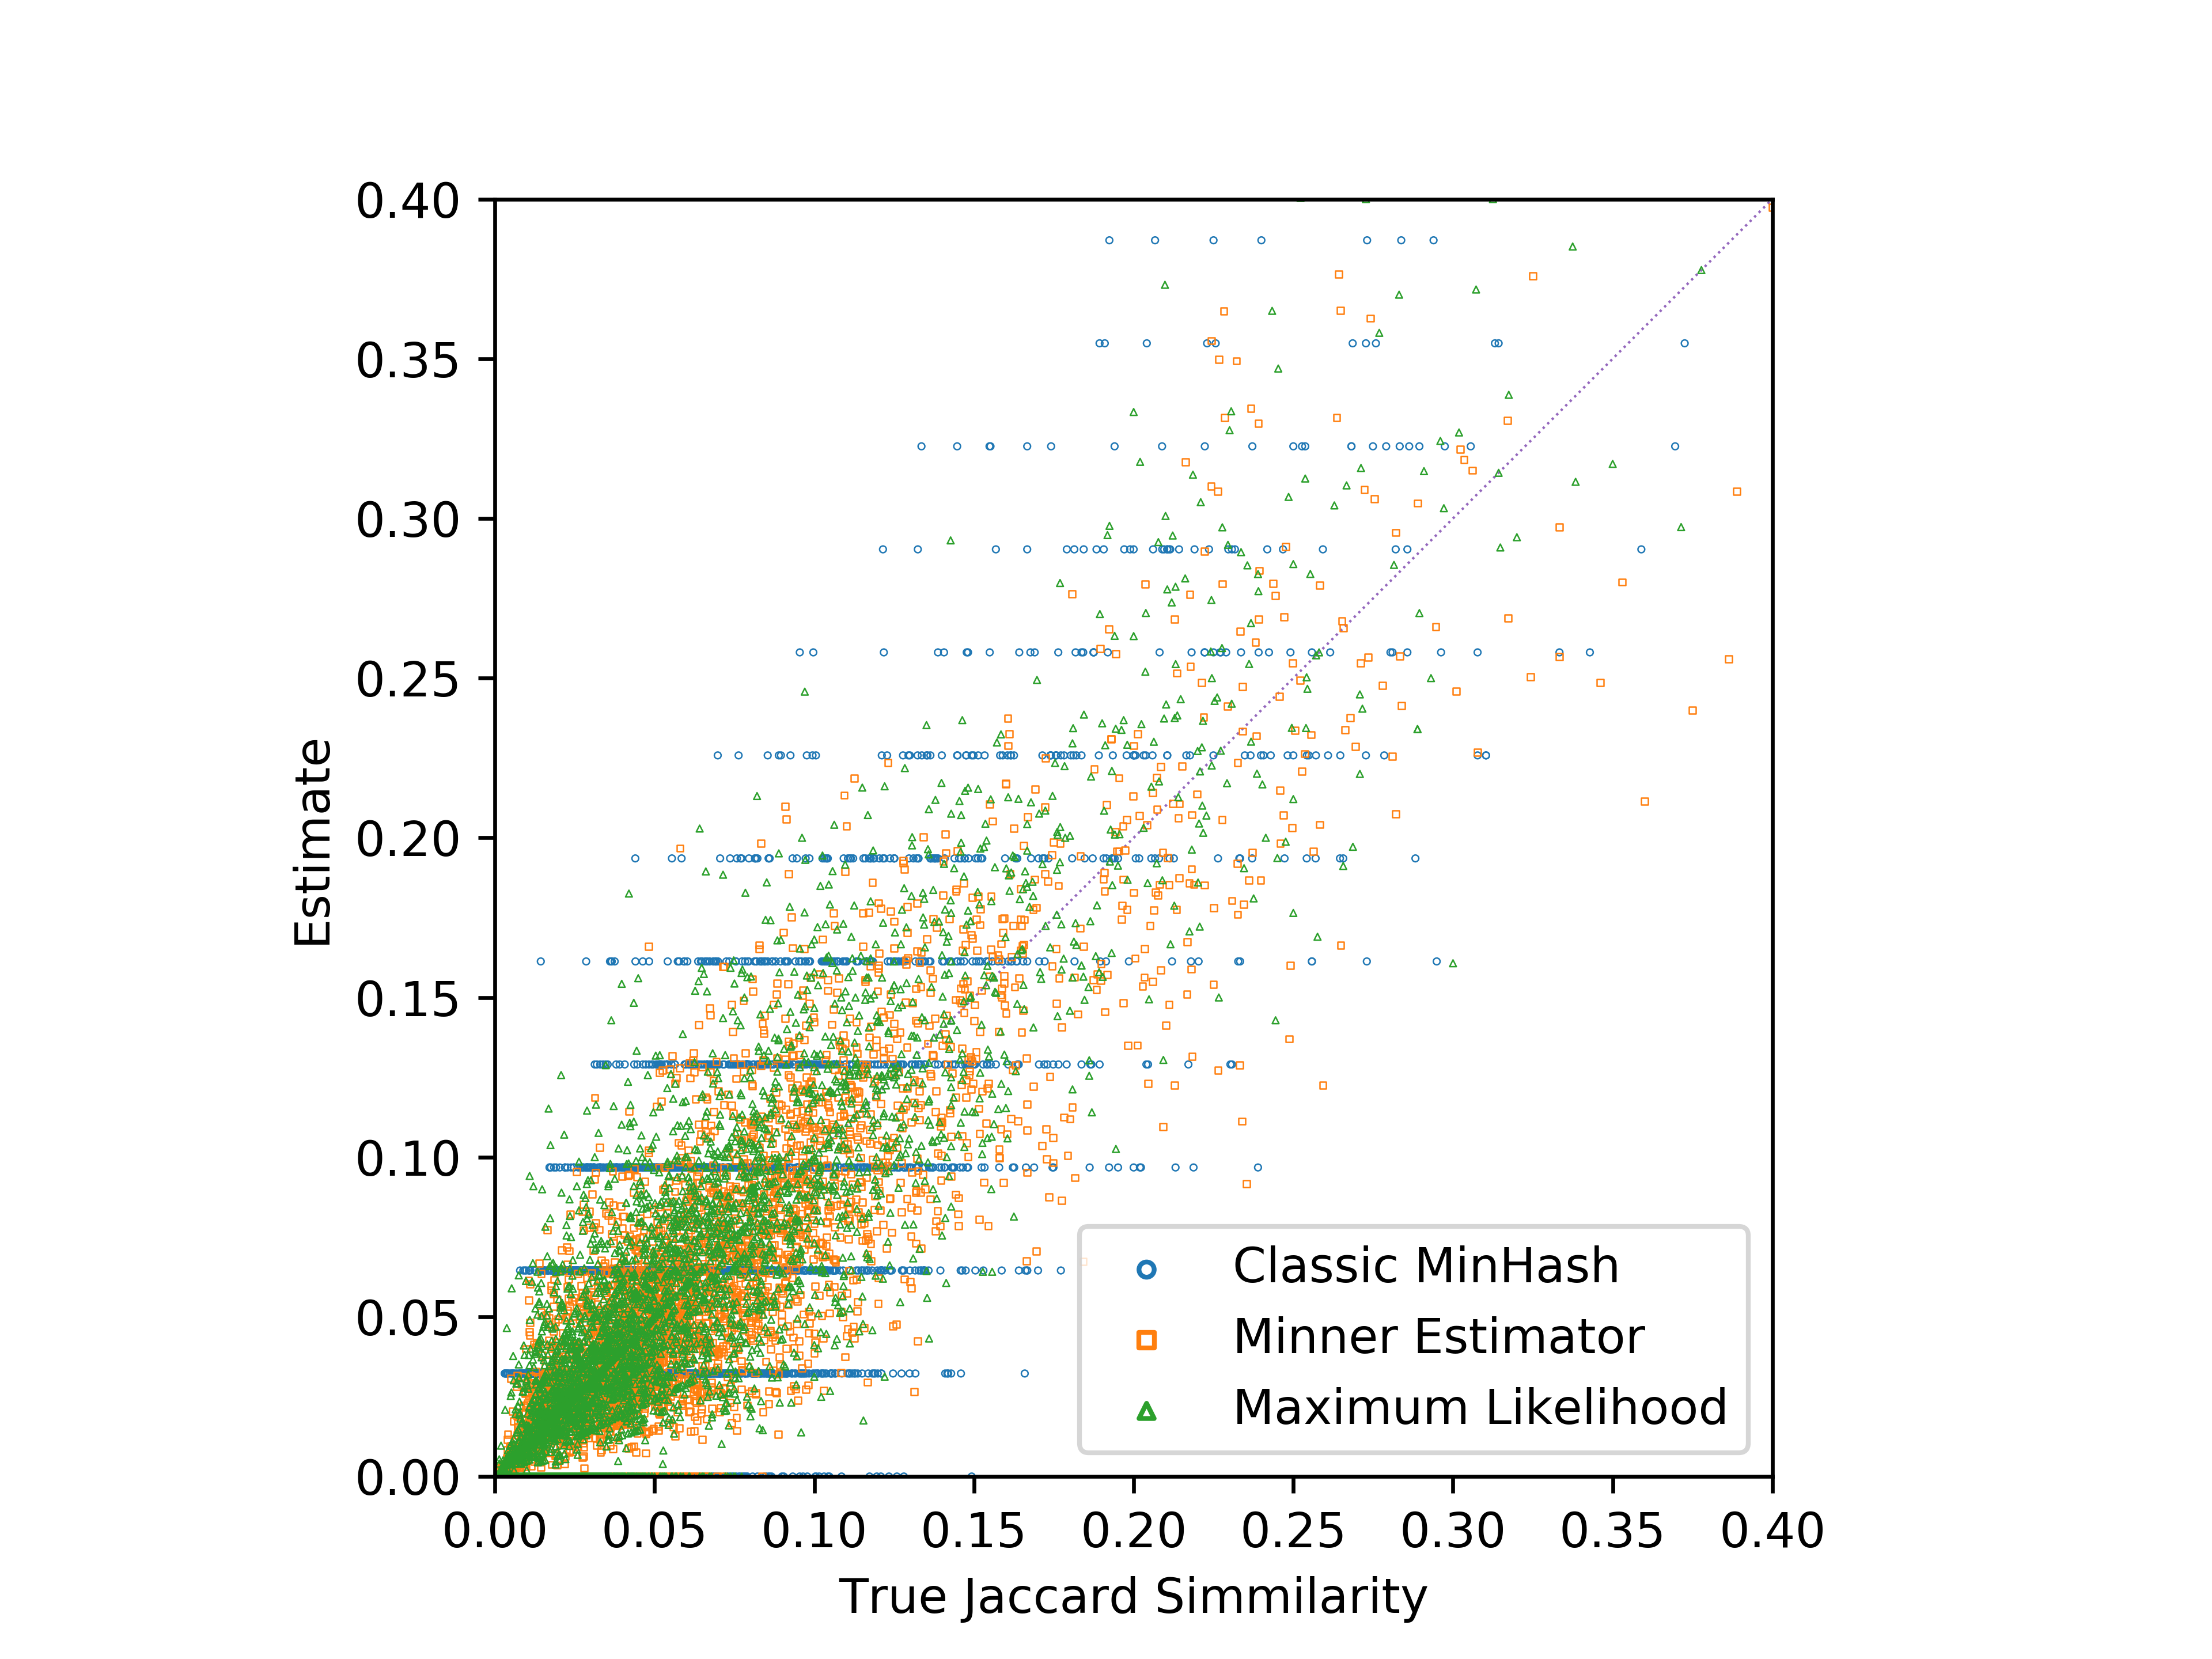
\includegraphics[trim=10 0 10 30,clip,width=\linewidth]{figures/scatter}
   \caption{Typical query in the Netflix dataset with 5,000 pairs, using $K=31$.
      The Classical Estimator shows clear banding, due to it taking only $K$ different values.
   }
   \label{fig:scatter}
\end{figure}

There is no clear answer as to which of the new estimators are best.
The Minner estimator with newton=8 can sometimes give results quite different from MLE, because of the approximation into making it linear.

It's not always clear which 

TODO:
• Discuss results
• Explain conflicting results, unexpected findings and discrepancies with other research
   - Uhm..
• State limitations of the study
• State importance of findings

\section{Open Problems}

Can we also better estimate other types of MinHash?
\begin{enumerate}
   \item Weighted MinHash
   \item $b$-bit MinHash
   \item Bottom-$k$ MinHash
   \item Find the best sketch for sets in general. Like how Supermajorities is best for queries.
   \item Use a prior better than uniform for $Y$.
      One might for example take into account skew distributions, where some tokens are more likely than other.
   \item Can we show the Minner Estimator is unbiased? Is seems unbiased, but is it?
      Can we prove anything else about it, or maybe improve it?
\end{enumerate}

%\begin{acks}
%Rasmus Pagh and Ninh Pahm
%\end{acks}

